\documentclass[aps,preprint,amsmath,amssymb]{revtex4-1}

\usepackage{graphicx}
\usepackage{epsfig}
\usepackage{bm}
\usepackage{color}
\usepackage{float}
\usepackage{dcolumn}
\usepackage{subfigure}
\usepackage{multirow} 


\begin{document}

\title{Third order onebody diagrams}


\author{ } 

\begin{abstract} 
All diagrams to third order in the interaction for an arbitrary two-body interaction $\hat{v}$.
\end{abstract}

%\pacs{02.70.Ss, 31.15.A-, 31.15.bw, 71.15.-m, 73.21.La}

\maketitle

\section*{Expressions}
The states $pq$ represent outgoing single-particle states. They can be either hole or particle states.
Holes states are labeled as $ijk\dots$ and particle states are $abc\dots$, the standard quantum chemistry notation. 
\subsection*{Diagram 1-5}
\[
\frac{1}{4}\sum_{abcd}\sum_{i}\frac{\langle pi| \hat{v} |ab  \rangle \langle ab| \hat{v} |cd  \rangle \langle cd| \hat{v} |qi  \rangle }{(\varepsilon_q+\varepsilon_i-\varepsilon_c-\varepsilon_d) (\varepsilon_q+\varepsilon_i-\varepsilon_a-\varepsilon_b)}.
\]

\subsection*{Diagram 1-6}
\[
-\frac{1}{4}\sum_{abc}\sum_{ij}\frac{\langle pc| \hat{v} |ab  \rangle \langle ab| \hat{v} |ij  \rangle \langle ij| \hat{v} |cq  \rangle }{(\varepsilon_i+\varepsilon_j-\varepsilon_a-\varepsilon_b) (\varepsilon_i+\varepsilon_j-\varepsilon_p-\varepsilon_c)}.
\]
\subsection*{Diagram 1-7}
\[
\frac{1}{4}\sum_{abc}\sum_{ij}\frac{\langle pc| \hat{v} |ij  \rangle \langle ij| \hat{v} |ab  \rangle \langle ab| \hat{v} |cq  \rangle }{(\varepsilon_i+\varepsilon_j-\varepsilon_p-\varepsilon_c) (\varepsilon_i+\varepsilon_j+\varepsilon_q-\varepsilon_a-\varepsilon_p-\varepsilon_b)}.
\]

\subsection*{Diagram 1-8}
\[
-\frac{1}{4}\sum_{a}\sum_{ijkl}\frac{\langle ij| \hat{v} |qa  \rangle \langle kl| \hat{v} |ij  \rangle \langle pa| \hat{v} |kl  \rangle }{(\varepsilon_k+\varepsilon_l-\varepsilon_p-\varepsilon_a) (\varepsilon_i+\varepsilon_j-\varepsilon_a-\varepsilon_p)}.
\]


\subsection*{Diagram 1-9}
\[
-\frac{1}{4}\sum_{ab}\sum_{ijk}\frac{\langle jp| \hat{v} |ab  \rangle \langle ab| \hat{v} |ik  \rangle \langle ik| \hat{v} |qj  \rangle }{(\varepsilon_k+\varepsilon_i-\varepsilon_a-\varepsilon_b) (\varepsilon_q+\varepsilon_j-\varepsilon_a-\varepsilon_b)}.
\]


\subsection*{Diagram 1-10}
\[
-\frac{1}{4}\sum_{ab}\sum_{ijk}\frac{\langle ab| \hat{v} |qk  \rangle \langle kp| \hat{v} |ij  \rangle \langle ij| \hat{v} |ab  \rangle }{(\varepsilon_k+\varepsilon_q-\varepsilon_a-\varepsilon_b) (\varepsilon_q+\varepsilon_j+\varepsilon_i-\varepsilon_a-\varepsilon_b-\varepsilon_p)}.
\]


\subsection*{Diagram 1-11}
\[
-\frac{1}{2}\sum_{ab}\sum_{ijk}\frac{\langle ab| \hat{v} |kj  \rangle \langle pk| \hat{v} |qi  \rangle \langle ij| \hat{v} |ab  \rangle }{(\varepsilon_k+\varepsilon_j-\varepsilon_a-\varepsilon_b) (\varepsilon_q+\varepsilon_j+\varepsilon_i-\varepsilon_a-\varepsilon_b-\varepsilon_p)}.
\]


\subsection*{Diagram 1-12}
\[
\frac{1}{2}\sum_{abc}\sum_{ij}\frac{\langle cb| \hat{v} |ij  \rangle \langle ij| \hat{v} |ab  \rangle \langle pa| \hat{v} |qc  \rangle }{(\varepsilon_i+\varepsilon_j-\varepsilon_a-\varepsilon_c) (\varepsilon_q+\varepsilon_j+\varepsilon_i-\varepsilon_a-\varepsilon_b-\varepsilon_p)}.
\]

\subsection*{Diagram 1-13}
\[
\frac{1}{2}\sum_{abc}\sum_{ij}\frac{\langle ab| \hat{v} |ij  \rangle \langle ic| \hat{v} |ab  \rangle \langle jp| \hat{v} |cq  \rangle }{(\varepsilon_i+\varepsilon_j-\varepsilon_a-\varepsilon_b) (\varepsilon_j-\varepsilon_c)}.
\]

\subsection*{Diagram 1-14}
\[
\frac{1}{2}\sum_{abc}\sum_{ij}\frac{\langle pc| \hat{v} |qi  \rangle \langle ab| \hat{v} |cj  \rangle \langle ij| \hat{v} |ab  \rangle }{(\varepsilon_i+\varepsilon_q-\varepsilon_p-\varepsilon_c) (\varepsilon_q+\varepsilon_j+\varepsilon_i-\varepsilon_a-\varepsilon_b-\varepsilon_p)}.
\]

\subsection*{Diagram 1-15}
\[
-\frac{1}{2}\sum_{ab}\sum_{ijk}\frac{\langle kp| \hat{v} |bq  \rangle \langle ij| \hat{v} |ak  \rangle \langle ab| \hat{v} |ij  \rangle }{(\varepsilon_i+\varepsilon_j-\varepsilon_a-\varepsilon_b) (\varepsilon_k-\varepsilon_b)}.
\]

\subsection*{Diagram 1-16}
\[
-\frac{1}{2}\sum_{ab}\sum_{ijk}\frac{\langle pa| \hat{v} |qk  \rangle \langle kb| \hat{v} |ij  \rangle \langle ij| \hat{v} |ab  \rangle }{(\varepsilon_q+\varepsilon_k-\varepsilon_p-\varepsilon_a) (\varepsilon_q+\varepsilon_j+\varepsilon_i-\varepsilon_a-\varepsilon_b-\varepsilon_p)}.
\]

\subsection*{Diagram 1-17}
\[
\sum_{abc}\sum_{ij}\frac{\langle ac| \hat{v} |ij  \rangle \langle jb| \hat{v} |cq  \rangle \langle ip| \hat{v} |ab \rangle }{(\varepsilon_i+\varepsilon_j-\varepsilon_a-\varepsilon_c) (\varepsilon_q+\varepsilon_i-\varepsilon_a-\varepsilon_b)}.
\]

\subsection*{Diagram 1-18}
\[
\sum_{abc}\sum_{ij}\frac{\langle ij| \hat{v}| ab  \rangle \langle bp| \hat{v} |jc  \rangle \langle ac| \hat{v} |iq  \rangle }{(\varepsilon_i+\varepsilon_q-\varepsilon_a-\varepsilon_c) (\varepsilon_q+\varepsilon_j+\varepsilon_i-\varepsilon_a-\varepsilon_b-\varepsilon_p)}.
\]

\subsection*{Diagram 1-19}
\[
\sum_{abc}\sum_{ij}\frac{\langle pi| \hat{v} |ab  \rangle \langle jb| \hat{v} |ci  \rangle \langle ac| \hat{v} |qj  \rangle }{(\varepsilon_q+\varepsilon_j-\varepsilon_a-\varepsilon_c) (\varepsilon_q+\varepsilon_i-\varepsilon_a-\varepsilon_b)}.
\]


\subsection*{Diagram 1-20}
\[
-\sum_{ab}\sum_{ijk}\frac{\langle pb| \hat{v} |ik  \rangle \langle ka| \hat{v} |bj  \rangle \langle ij| \hat{v} |qa  \rangle }{(\varepsilon_i+\varepsilon_k-\varepsilon_p-\varepsilon_b) (\varepsilon_j+\varepsilon_i-\varepsilon_a-\varepsilon_p)}.
\]


\subsection*{Diagram 1-21}
\[
-\sum_{ab}\sum_{ijk}\frac{\langle ij| \hat{v} |aq  \rangle \langle kp| \hat{v} |bj  \rangle \langle ab| \hat{v} |ik  \rangle }{(\varepsilon_i+\varepsilon_k-\varepsilon_a-\varepsilon_b) (\varepsilon_j+\varepsilon_i-\varepsilon_a-\varepsilon_p)}.
\]



\subsection*{Diagram 1-22}
\[
-\sum_{ab}\sum_{ijk}\frac{\langle ap| \hat{v} |ik  \rangle \langle bk| \hat{v} |jq  \rangle \langle ij| \hat{v} |ab  \rangle }{(\varepsilon_i+\varepsilon_k-\varepsilon_a-\varepsilon_p) (\varepsilon_q+\varepsilon_j+\varepsilon_i-\varepsilon_a-\varepsilon_b-\varepsilon_p)}.
\]

\begin{figure}%[hbtp]
     \begin{center}
            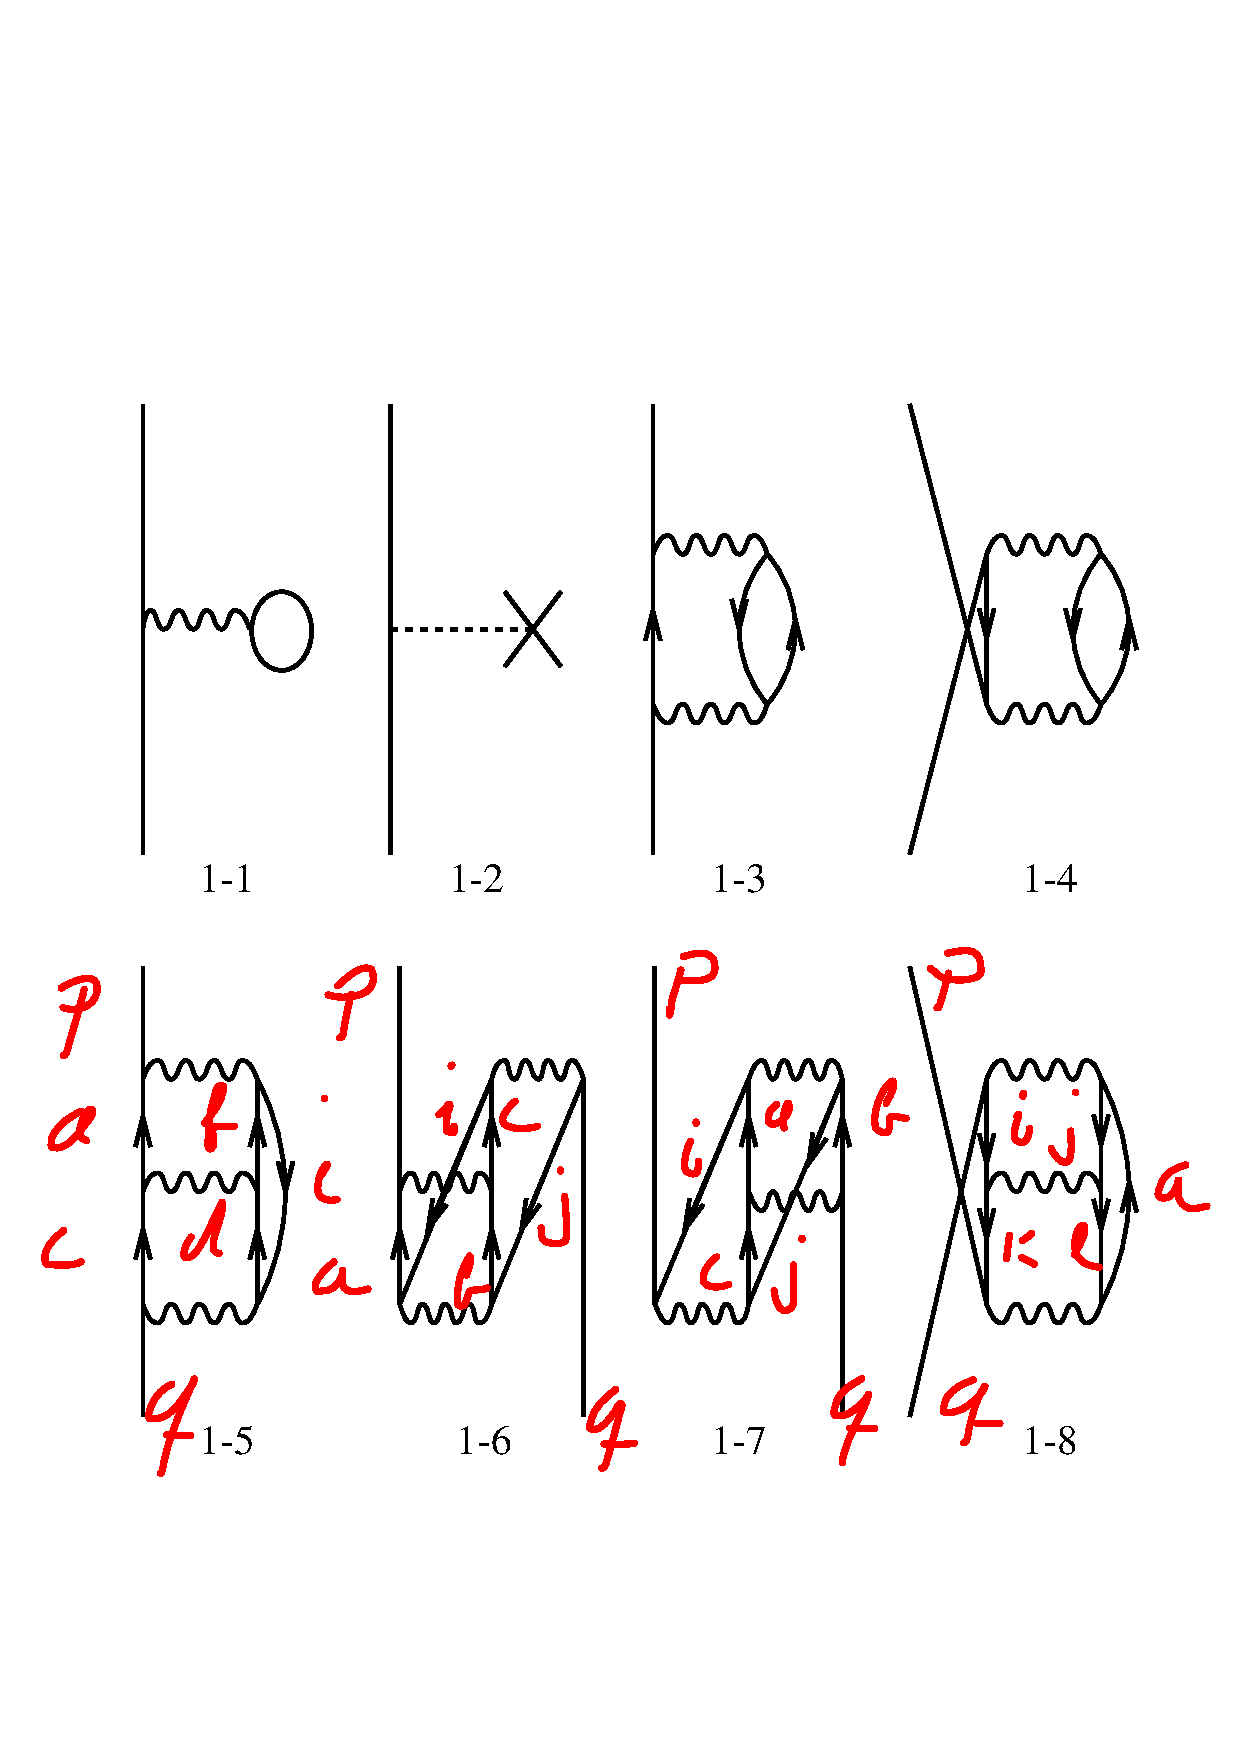
\includegraphics[width=0.38\textwidth]{onebd1.pdf}
            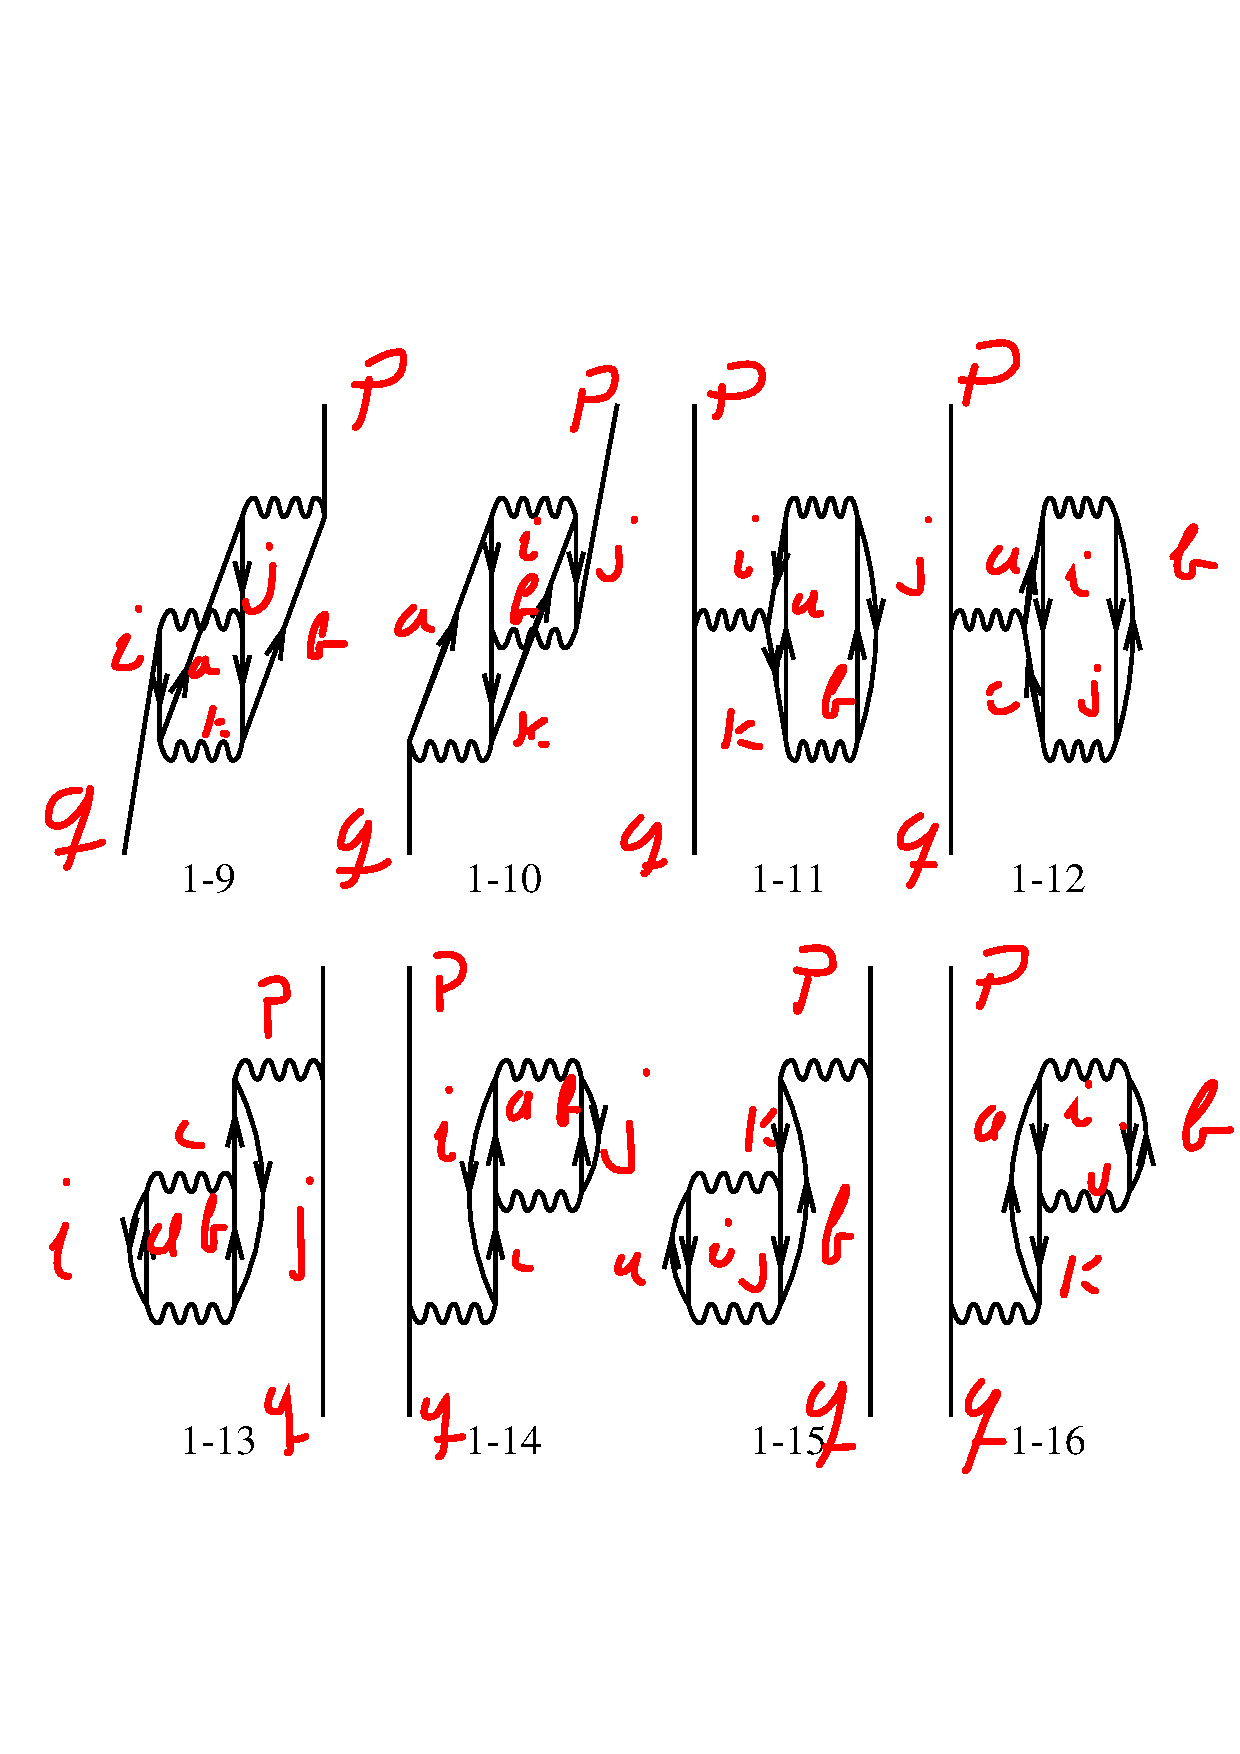
\includegraphics[width=0.38\textwidth]{onebd2.pdf}
            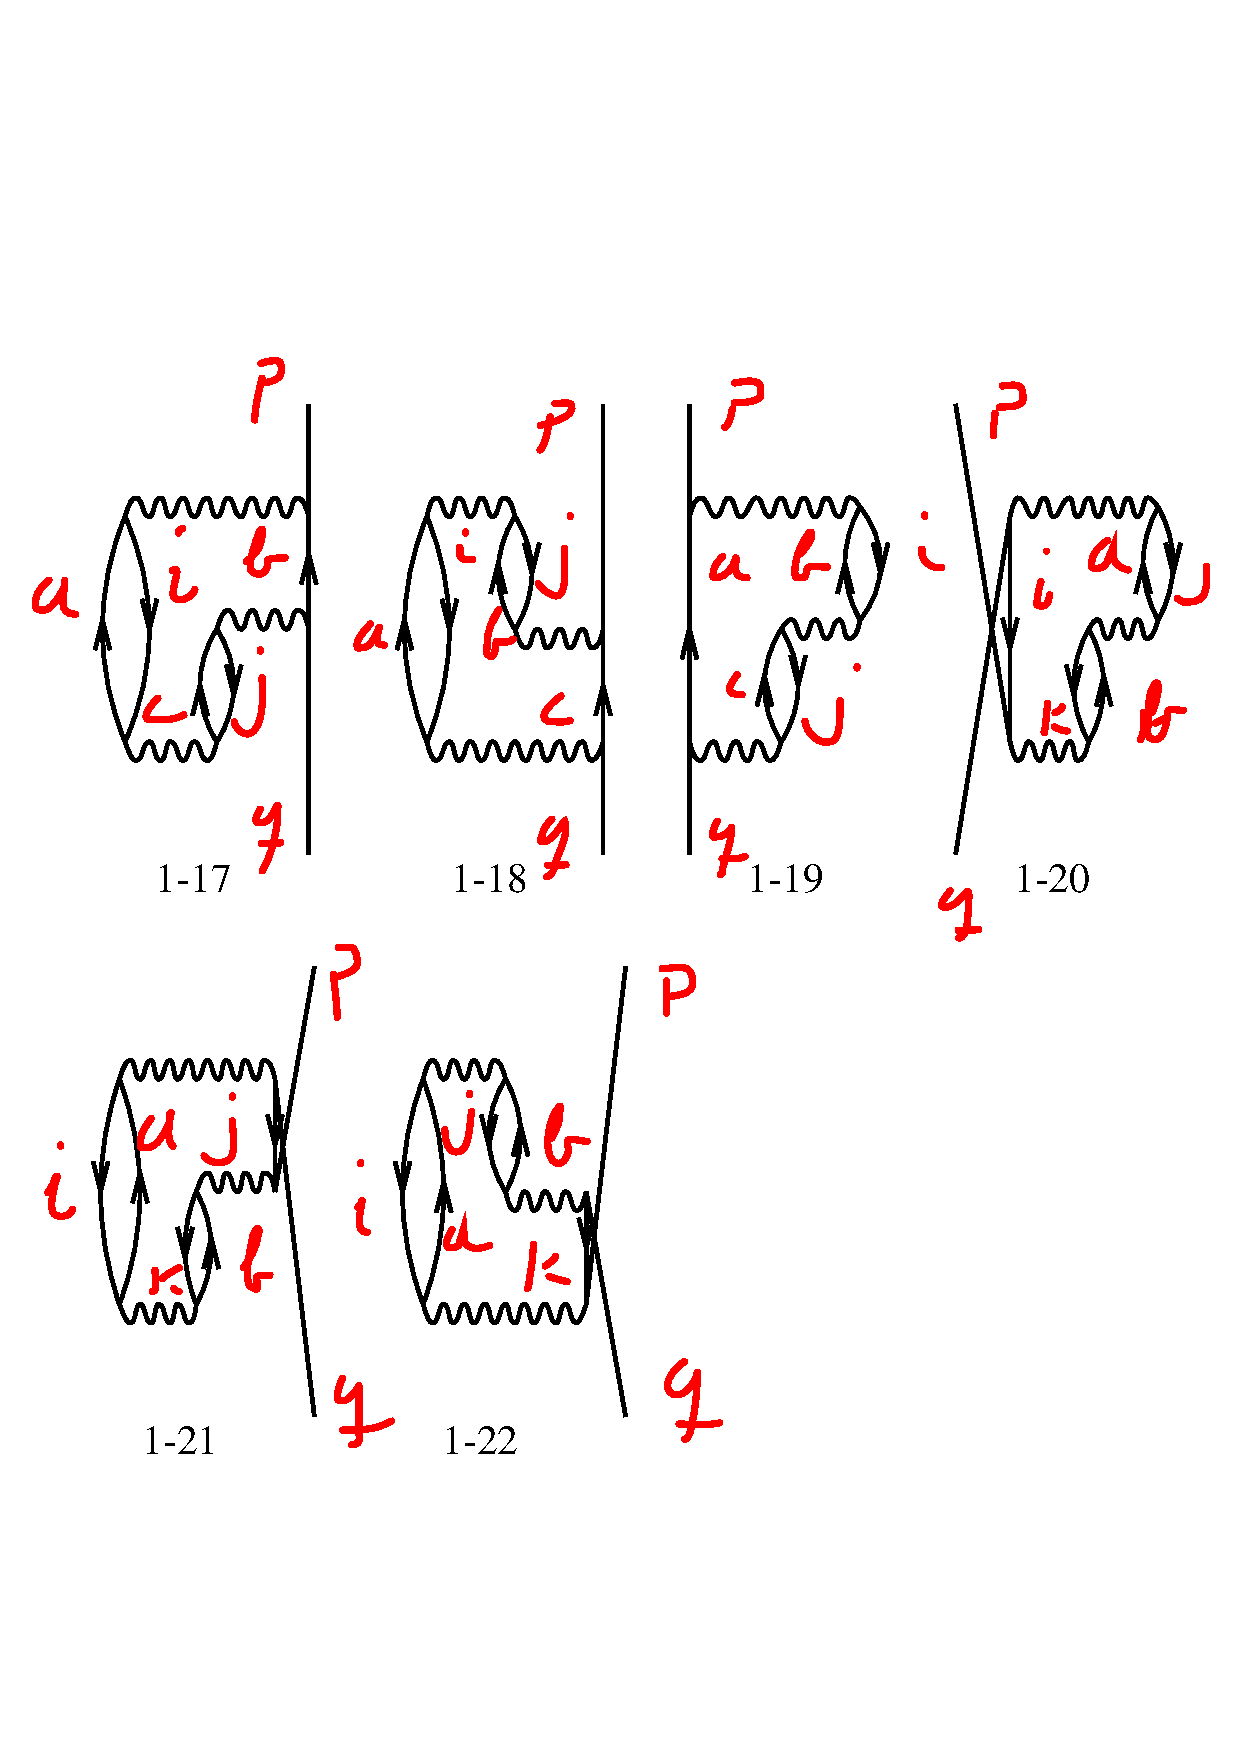
\includegraphics[width=0.38\textwidth]{onebd3.pdf}
    \end{center}
    \caption{One-body diagrams to third order in the interaction.}
\end{figure}


\end{document}




